\section{Triangulation system geometry}
\label{sec:init-modelanalysis}
At first, we analyse the errors due to the geometry of the triangulation system. For simplicity, we will focus on the standard geometry (described in Section \ref{sec:lctt}): the analysis for other geometries is trivial. \\

As illustrated in Figure \ref{fig:laser-triang}, the laser-camera pair form a triangle with angle $\phi$ between the baseline (the plane along the distance between the laser and the camera), and the optical axis of the camera. In \acs{SOL} systems, $\phi$ is
\clearpage
  \begin{figure}[h]
    \centering
    \begin{minipage}[c]{\textwidth}
      \centering
      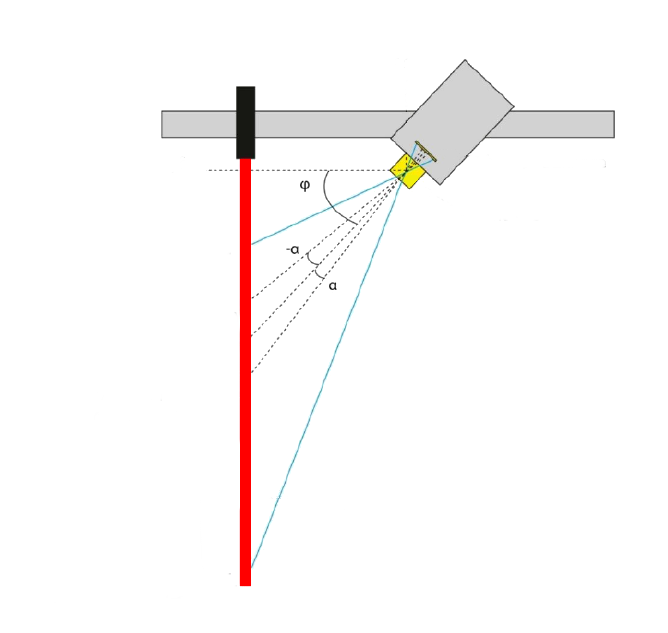
\includegraphics[width=0.7\textwidth]{./images/model/laser_triang.png}
      \caption{\acs{FOV} and characteristic angles}
      \label{fig:laser-triang}
    \end{minipage}
    \vfill
    \begin{minipage}[c]{\textwidth}
      \centering
      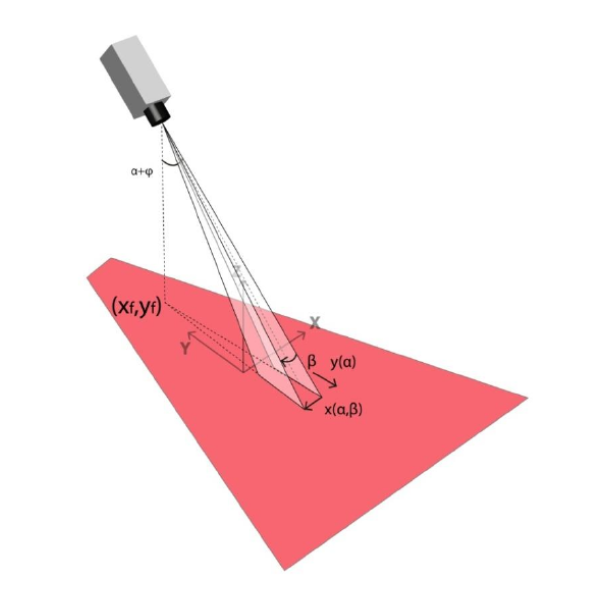
\includegraphics[width=0.7\textwidth]{./images/model/laser_triang_pdv.png}
      \caption{Angles definitions}
      \label{fig:laser-triang-pdv}
    \end{minipage}
  \end{figure}
\clearpage \noindent
called \textit{triangulation angle}. If $\phi$ and the baseline are known, any point in the 3D space belonging to the laser plane, is located estimating the offset $\alpha$ with respect to $\phi$, and the offset $\beta$ with respect to the optical axis of the camera. Accordingly with \cite{th:quattrini}, and using simple mathematical relations, we can locate the $y$ coordinate as function of the angle $\alpha$ as follows:
  \begin{equation}
    \label{eq:model-ya}
    y\left( \alpha \right) = y_f + z_f \tan \left( \phi + \alpha \right)
  \end{equation}
where $\left( x_f, y_f, z_f \right)$ are the principal point projection coordinates in the laser plane (in the world reference system), as shown in Figure \ref{fig:laser-triang-pdv}. Note that using this notation, $z_f$ is the distance from the laser to the camera, previously called baseline. \\

Now let's look at the Figure \ref{fig:laser-triang-pdv}. As mentioned at the end of the Section \ref{sec:lctt}, camera's resolutions varies changing the distance of the target from the camera. In particular this is true for the resolution along the laser line (axis $x$ with respect to out notation). Points having the same $x$ coordinates but different $y$ are estimated with different camera resolutions. This means that the values of $x$ strongly depends on the angle $\beta$ (that identify the value of $x$ with respect the the optical axis of the camera), but also on the angle $\alpha$ (that identifies the value of $y$ with respect to the triangulation angle). For these reasons we can write
  \begin{equation}
  \label{eq:model-xab}
    x(\alpha, \beta) = \frac{y\left( \alpha \right) - y_f}{\sin(\phi + \alpha)}\tan(\beta)
  \end{equation} \\
As we can see, $x$ strongly depends on $y$, accordingly with what we said in Section \ref{sec:lctt}, about the trapezoidal shape of the laser plane. Still for the shape of the laser, a similar consideration can be made for the $y$ coordinate, because of the trapezoidal shape of the laser plane.
% To be precise, a similar consideration can be made for the $y$ coordinate, because of the trapezoidal shape of the laser plane.
However, in this case the differences between the nearest and the farthest \acs{FOV}s along the $x$ axis, are negligible. For theses reasons we will consider Equation \ref{eq:model-ya} as a good approximation of the relation between $y$ and $\alpha$. \\

Accordingly with what we said in Section \ref{sec:teo-calibration}, during calibration phase the choice of the reference system is arbitrary, so we can put $\left( x_f, y_f, z_f \right) = \left( 0, 0, z_f \right)$ without loss of generality. In this way, Equations \ref{eq:model-ya} and \ref{eq:model-xab} can be simplified. \\

At this point it is easy to estimate the error associated with the two newly introduced measures. Applying the simplification, for Equation \ref{eq:model-ya} we can write:
  \begin{equation}
    \label{eq:model-ya-err0}
    \sigma_{y_\alpha} = \sqrt{
      \left( \frac{\partial y}{\partial z_f} \right)^2 \sigma_{z_f}^2 +
      \left( \frac{\partial y}{\partial \phi} \right)^2 \sigma_\phi^2 +
      \left( \frac{\partial y}{\partial \alpha} \right)^2 \sigma_\alpha^2
    }
  \end{equation}
while for Equation \ref{eq:model-xab} we can write
  \begin{equation}
    \label{eq:model-xab-err0}
    \sigma_{x\left( \alpha, \beta \right)} = \sqrt{
      \left( \frac{\partial x}{\partial \phi} \right)^2 \sigma_\phi^2 +
      \left( \frac{\partial x}{\partial \alpha} \right)^2 \sigma_\alpha^2 +
      \left( \frac{\partial x}{\partial \beta} \right)^2 \sigma_\beta^2
    }
  \end{equation}\\
In these last equations, the $\sigma$ are the errors committed evaluating each component in the Equations \ref{eq:model-ya} and \ref{eq:model-xab}. As we can see, in Equations \ref{eq:model-ya-err0} and \ref{eq:model-xab-err0} we are considering also $\phi$ and $z_f$ that are constructive parameters that depend on the accuracy with which the system was built or installed. Typically, these parameters are corrected thanks to the calibration process, that allows to estimate camera intrinsic and extrinsic parameters, as mentioned in Section \ref{sec:teo-calibration}. In addition, the calibration process uses many algorithms that in turn use different heuristics to estimate camera parameters. This means that all parameters are affected by error, but as we can see later, we can consider these errors negligible. So we can simplify Equations \ref{eq:model-ya-err0} and \ref{eq:model-xab-err0} respectively as follows
  \begin{equation}
    \label{eq:model-ya-err1}
    \sigma_{y_\alpha} = \sqrt{
      \left( \frac{\partial y}{\partial \alpha} \right)^2 \sigma_\alpha^2
    }
  \end{equation}
  
  \begin{equation}
    \label{eq:model-xab-err1}
    \sigma_{x\left( \alpha, \beta \right)} = \sqrt{
      \left( \frac{\partial x}{\partial y_\alpha} \right)^2 \sigma_{y_\alpha}^2 +
      \left( \frac{\partial x}{\partial \alpha} \right)^2 \sigma_\alpha^2 +
      \left( \frac{\partial x}{\partial \beta} \right)^2 \sigma_\beta^2
    }
  \end{equation} \\

Keeping focus on the geometry of the system, the second element to consider is the laser plane. In standard geometry, variations on laser pitch and roll rotations, with respect to the reference system, can affect heavily the final measure. By trigonometry we know that by changing the angle, the point projections also change in the two axes of the reference system. The same effect is present when we rotate the laser plane with respect to the $x$ axis (roll) or with respect to the $y$ axis (pitch). These errors are more apparent in the other triangulation geometries. What we have to do, is to compensate these rotations projecting the laser plane on the ideal one. The compensations are performed as follows:
  \begin{equation}
    \begin{matrix}
      y_w = y(\alpha) \cdot cos(\rho) \\ ~ \\
      x_w = x(\alpha, \beta) \cdot \cos(\gamma)
    \end{matrix}
    \label{eq:radial-compensations}
  \end{equation} \\
where $\rho$ is the laser roll angle, and $\gamma$ is the laser pitch angle. Using the model introduced in Equation \ref{eq:er_prop_2}, we can write, respectively:
  \begin{equation}
    \sigma_{y_w} = \sqrt{
      \left( \frac{\partial y_w}{\partial y(\alpha)} \right)^2 \sigma_{y_\alpha}^2
      + \left( \frac{\partial y_w}{\partial \rho} \right)^2 \sigma_\rho^2
    }
    \label{eq:err-radial-comp-yw}
  \end{equation}
  \begin{equation}
    \sigma_{x_w} = \sqrt{
      \left( \frac{\partial x_w}{\partial x\left( \alpha, \beta \right)} \right)^2 \sigma_{x\left( \alpha, \beta \right)}^2 +
      \left( \frac{\partial x_w}{\partial \gamma} \right)^2 \sigma_\gamma^2
    }
    \label{eq:err-radial-comp-xw}
  \end{equation} \\
where $\sigma_{y_\alpha}$ and $\sigma_{x\left( \alpha, \beta \right)}$ are the ones evaluated in Equations \ref{eq:model-ya-err1} and \ref{eq:model-xab-err1} respectively. \\

A practical example in which these compensations are needed, is the \acs{WPMS}. In autonomous \acs{WPMS}s placed alongside the rails, specular geometry is generally used, and wheels are measured while the train is running. In these cases we are not sure to measure the wheel exactly along its axis, so the acquired profiles have to be compensated. This type of correction is called \textit{radial compensation}. \\
% The errors due to non-ideality of laser plane placement can be seen also as non-ideality of work conditions. In autonomous \acs{WPMS}s placed alongside the rails, specular geometry is generally used, and wheels are measured while the train is running. In these cases we are not sure to measure the wheel exactly along its axis, and typically corrections like the ones for rolls are needed. In these field, these corrections are referred as \textit{radial compensation}. \\
We can consider the same things about pitch. Sometimes the wheel under analysis is not perpendicular with the laser plane, because wheel yaw and camber. Also in these cases $x$ values must be compensated.

%We can see here, the determination of $x$ is fully dependent by the formulation on $y$.
